\section{Saving user preferences}\label{sec:saving-user-preferences}

To make our program more user-friendly, we want to be able to store a users preferences on climate, price,
time, and so on.
This will be stored locally in a configuration file, which we will call
``\verb|preferences.json|''.
As the name suggests we have chosen to store the data in a JSON format, this is partly because we already have
a system in place in order to store JSON data, but also because it allows us to access individual keys of data such as
``price''.
If implemented correctly storing the preferences as JSON also allows us to remove or add different keys to the file
later if it is needed, but at this point we only need to save four keys called: price, time, environment and health.

For the actual implementation for saving the file.
We will, if the program is executed, always require data for all our chosen preference categories.
A way to do this is to, at the programs start, initialize the save file with some standard data, so the program can
continue running even if the user does not want to input their own preferences.
We initialize the save file through a function called ``InitializePreferenceFile''

\begin{figure}
    \centering
    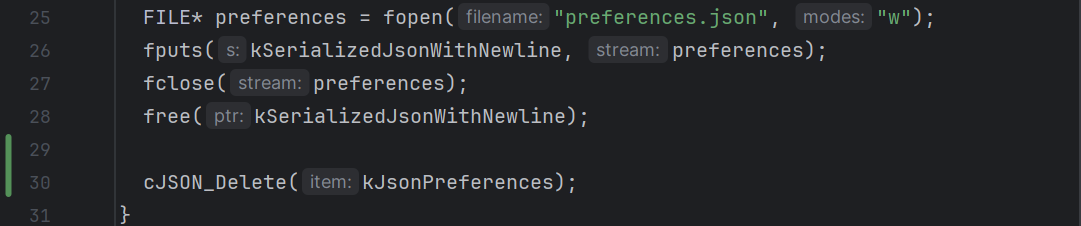
\includegraphics[width=\textwidth]{InitPref}
    \caption{Saving preferences to file.}
    \label{fig:figureInitSaveFile}
\end{figure}

In Figure~\ref{fig:figureInitSaveFile} it can be seen that we are trying to open the preferences file,
and by using ``fopen'' we make use of the property that creates the file if it does not already exist.
The rest of the code inside InitializePreferenceFile is used to convert our given inputs into the JSON format, which in
C is somewhat difficult.

The remaining functions for the preference file are SetUserPreference and GetUserPreference.
The SetUserPreference function will work by taking in two inputs, a key and a value for that key.
This would be written as \(SetUserPreference("key", value)\).
When we want to change the values in the JSON file through C, we must first read the file and then parse it as cJSON[.]
In this way we can actually make the changes to the stored values.
Parsing JSON and generating JSON is done through the library cJSON which we have chosen to use.
As seen above it works by first parsing the content of the preference file and then searching for the item we want to
change.

\begin{figure}
    \centering
    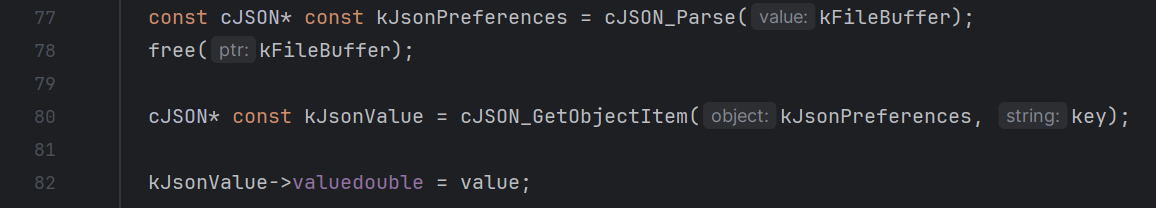
\includegraphics[width=\textwidth]{ParsingJSON}
    \caption{Parsing JSON.}
    \label{fig:figureParsingJSON}
\end{figure}

cJSON stores all JSON values as structs and to change the value we access the struct as seen on line 82 in
Figure~\ref{fig:figureParsingJSON}.
The next step is then to save the changes to our preferences file, but because saving to a file in C can get
complicated if you change the length of the file, we sidestep this problem by overwriting the whole save file with the
updated values.

Finally, the last step is to read the file, so we can use the stored data in our program.
This is done much in the same way we used in SetUserPreference as we open the file, parse the JSON and then access
the item we want to use.
Both InitializePreferenceFile and SetUserPreference are void functions, but GetUserPreference is a double function
this is done so the returned value will be the value for the preference we want to get out of the save file, see
Figure~\ref{fig:figureGetPref}.
GetUserPreference only takes in one input which is the key we want to look for, this could be ``price'' or another of
the attributes.

\begin{figure}
    \centering
    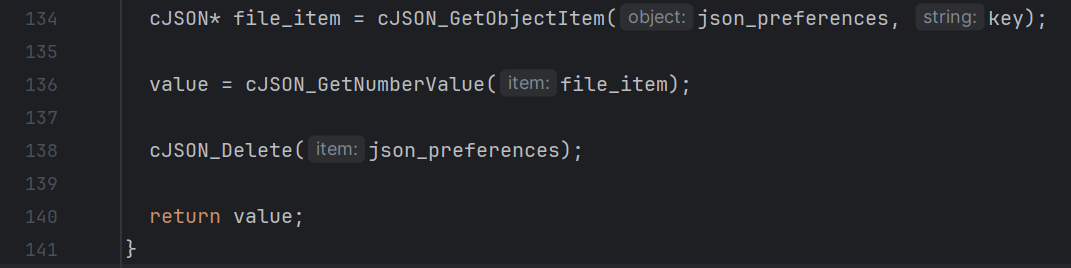
\includegraphics[width=\textwidth]{GetPref}
    \caption{Reading attribute value from preference file.}
    \label{fig:figureGetPref}
\end{figure}

With these three functions it is now possible for us to store and use preferences locally on the device.
